\chapter{Distributions of one Variable}


\section{Characterizing a Distribution}

\subsection{Distribution Center}
\subsubsection{Mean} \index{general}{mean}
By default, when we talk about the \emph{mean value} we mean the \emph{arithmetic mean} $\bar{x}$:

\begin{equation}
  \bar{x} = \frac{{\sum\limits_{i = 1}^n {{x_i}} }}{n}
\end{equation}

\subsubsection{Median} \index{general}{median}
The \emph{median} is that value that comes half-way when the data are ranked in order.
In contrast to the mean, it is not affected by outlying data points.

\subsubsection{Mode} \index{general}{mode}
The \emph{mode} value is the most frequently occurring value in a distribution.

\subsubsection{Geometric Mean}\index{general}{geometric mean}
In some situations the \emph{geometric mean} can be useful to describe the location of a distribution. It is usually close to the median, and can be calculated via the arithmetic mean of the log of the values.

\subsection{Quantifying Variability}\label{sec:centiles}

\subsubsection{Range}\index{general}{range}
This one is fairly easy: it is the difference between the highest and the lowest data value.
The only thing that you have to watch out for: after you have acquired your data, you have to check for \emph{outliers}, i.e. data points with a value much higher or lower than the rest of the data. Often, such points are caused by errors in the selection of the sample or in the measurement procedure. There are a number of tests to check for outliers. One of them is to check for data which lie more than 1.5*\emph{inter-quartile-range} (IQR) above or below the first/third quartile (see below).


\subsubsection{Centiles}\index{general}{centiles}\index{general}{percentiles}
While you won't often hear the expression \emph{centiles}, you will frequently encounter specific centiles, e.g. \emph{quartiles}, or the \emph{median value}. 

\begin{description}
  \item[Probability Density Function (PDF)]\index{general}{probability density function} The PDF, or density of a continuous random variable, is a function that describes the relative likelihood for this random variable to take on a given value.
  \item[Cumulative Density Function (CDF)]\index{general}{cumulative density function} Tells you for each value which percentage of the data has a lower value (Figure \ref{fig:CDF}).
  \item[Centile] Also called \emph{percentile}: The value below which a given percentage of the values occur. It corresponds to a value with a specified cumulative frequency.
\end{description}

For example, when you look for the data range which includes 95\% of the data, you have to find the $2.5^{th}$ and the $97.5^{th}$ percentile of your sample distribution.

The 50th percentile is the \emph{median}.

Also important are the \emph{quartiles}, i.e. the 25th and the 75th percentile. The difference between them is sometimes referred to as \emph{inter-quartile range (IQR)}\index{general}{IQR}.

Median, upper and lower quartile are used for the data display in box plots (Fig.\ref{fig:Boxplot}).

\begin{figure}[ht]
  \centering
  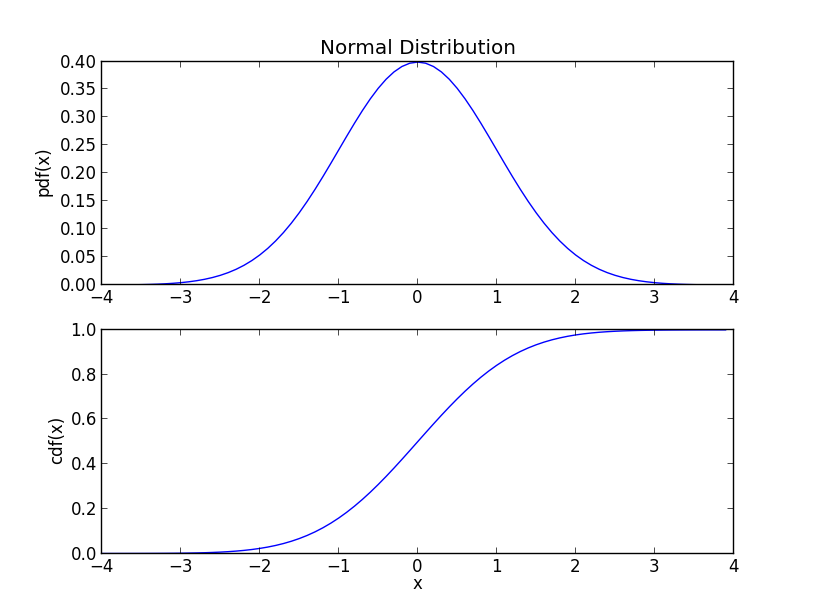
\includegraphics[width=0.5\textwidth]{../Images/NormalDist_PDF_CDF.png}\\
  \caption{\emph{Probability density function} (top) and \emph{Cumulative density function} (bottom) of a normal distribution.}\label{fig:CDF}
\end{figure}


\subsubsection{Standard Deviation and Variance}
The \emph{variance} (SD) of a distribution is defined as

\begin{equation}\label{eq_variance} \index{general}{variance}
  var = \frac{{\sum\limits_{i = 1}^n {({x_i-\bar{x}})^2} }}{n-1}
\end{equation}

Note that we divide by \emph{n-1} rather than the more obvious n: dividing by $n$ gives the variance of the observations around the sample mean, but we virtually always consider our data as a sample from some larger population and wish to use the sample data to estimate the variability in the population. Dividing by $n-1$ gives us a better estimate of the population variance.

The \emph{standard deviation} \index{general}{standard deviation} is simply given by the square root of the variance:

\begin{equation}
  s = \sqrt{var}
\end{equation}

In statistics it is often common to denote the population standard deviation with $\sigma$, and the sample standard deviation with $s$.

Watch out: in Python, by default the variance is calculated for "n". You have to set "ddof=1" to obtain the variance for "n-1":

\begin{lstlisting}
    In[19]: data = arange(7,14)

    In[20]: std(data, ddof=0)
    Out[20]: 2.0

    In[21]: std(data, ddof=1)
    Out[21]: 2.1602468994692865
\end{lstlisting}

\subsubsection{Standard Error} \index{general}{standard error}
While the standard deviation is a good measure for the distribution of your values, often you are more interested in the distribution of the mean value. For example, when you measure the response to a new medication, you might be interested in how well you can characterize this response, i.e. is how well you know the mean value. This measure is called the \emph{standard error of the mean}, or sometimes just the \emph{standard error}. In a single sample from a population with a standard deviation of $\sigma$ the variance of the sampling distribution of the mean is $\sigma^2/n$, and so the standard error of the mean is $\sigma/\sqrt{n}$.

For the \emph{sample standard error of the mean}, which is the one you will be working with most of the time, we have

\begin{equation}
  SE = \frac{s}{\sqrt{n}} = \sqrt{\frac{{\sum\limits_{i = 1}^n {({x_i-\bar{x}})^2} }}{n-1}} \cdot \frac{1}{\sqrt{n}}
\end{equation}

\subsection{Parameters Describing a Distribution}

\subsubsection{Location}

A \emph{location parameter} $x_0$  determines the "location" or shift of a distribution.

\begin{equation*}
  f_{x0}(x)=f(x-x_0)
\end{equation*}

Examples of location parameters include the mean, the median, and the mode.

\subsubsection{Scale}

The \emph{scale parameter} describes the width of a probability distribution.  If s is large, then the distribution will be more spread out; if s is small then it will be more concentrated. If the probability density exists for all values of $s$, then the density (as a function of the scale parameter only) satisfies

\begin{equation*}
   f_s(x) = f(x/s)/s,
\end{equation*}

where f is the density of a standardized version of the density.

\subsubsection{Shape Parameters}\index{general}{shape parameters}

A shape parameter is any parameter of a probability distribution that is neither a location parameter nor a scale parameter. If \emph{location }and \emph{shape} already completely determine the distribution (as is the case for e.g. the normal distribution or the exponential distribution, etc.), then these distributions don't have any \emph{shape parameter}. It follows that the \emph{skewness }and \emph{kurtosis} of these distribution are constants.


\subsubsection{Skewness}\index{general}{skewness}

Distributions are \emph{skewed} if they depart from symmetry. For example, if you have a measurement that cannot be negative, which is usually the case, then we can infer that the data have a skewed distribution if the standard deviation is more than half the mean. Such an asymmetry is referred to as \emph{positive skewness}. The opposite, negative skewness, is rare.


\begin{figure}
\centering
\begin{subfigure}{.5\textwidth}
  \centering
  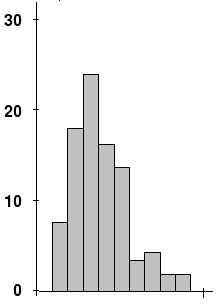
\includegraphics[width=0.4\textwidth]{../Images/SkewedDistribution.png}\\
  \caption{Example of experimental data with non-zero (positive) skewness.}
  \label{fig:skewness}
  \end{subfigure}%
\begin{subfigure}{.5\textwidth}
  \centering
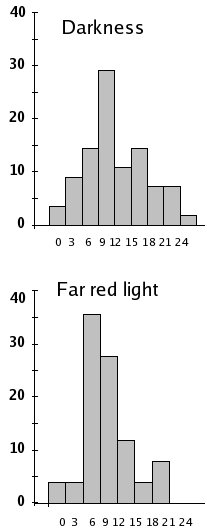
\includegraphics[width=0.3\textwidth]{../Images/KurtosisChanges.png}\\
  \caption{The "Darkness" data is platykurtic (−0.194), while "Far Red Light" shows leptokurtosis (0.055).}
  \label{fig:kurtosis}
  \end{subfigure}
\caption{Skew and Kurtosis of distributions (from Wikipedia).}
\label{fig:skewkurtosis}
\end{figure}


\subsubsection{Kurtosis}\index{general}{kurtosis}

Kurtosis is any measure of the "peakedness" of the probability distribution. Distributions with negative or positive excess kurtosis are called platykurtic distributions or leptokurtic distributions respectively.

\subsection{Central Limit Theorem}\index{general}{central limit theorem}
The central limit theorem states that for identically distributed independent random variables (also referred to as \emph{random variates})\index{general}{variate}, the mean of a sufficiently large number of these variables will be approximately normally distributed.

%(Lecture 5)

\section{Distribution Functions}

The variable for a standardized distribution function is often called \emph{statistic}\index{general}{statistic}. So you often find expressions like "the z-statistic" (for the normal distribution function), the "t-statistic" (for the t-distribution) or the "F-statistic" (for the F-distribution).

  \subsection{Probability and Samples}

  \subsection{Normal Distribution} \label{sec:normalDistribution}\index{general}{distributions!normal}

The \emph{Normal distribution} or \emph{Gaussian distribution} is by far the most important of all the distribution functions. This is due to the fact that the mean values of \emph{all} distribution functions approximate a normal distribution for large enough sample numbers.
Mathematically, the normal distribution is characterized by a mean value $\mu$, and a standard deviation $\sigma$:

\begin{equation}\label{eq_normal}
     f_{\mu,\sigma} (x) = \frac{1}{\sigma \sqrt{2 \pi}} e^{-( x - \mu )^2 /2 \sigma^2}
\end{equation}
where $ - \infty < x < \infty $, and $f_{\mu,\sigma}$ is the \emph{probability density function (PDF)} \index{general}{probability density function}.

\begin{figure}
  \centering
  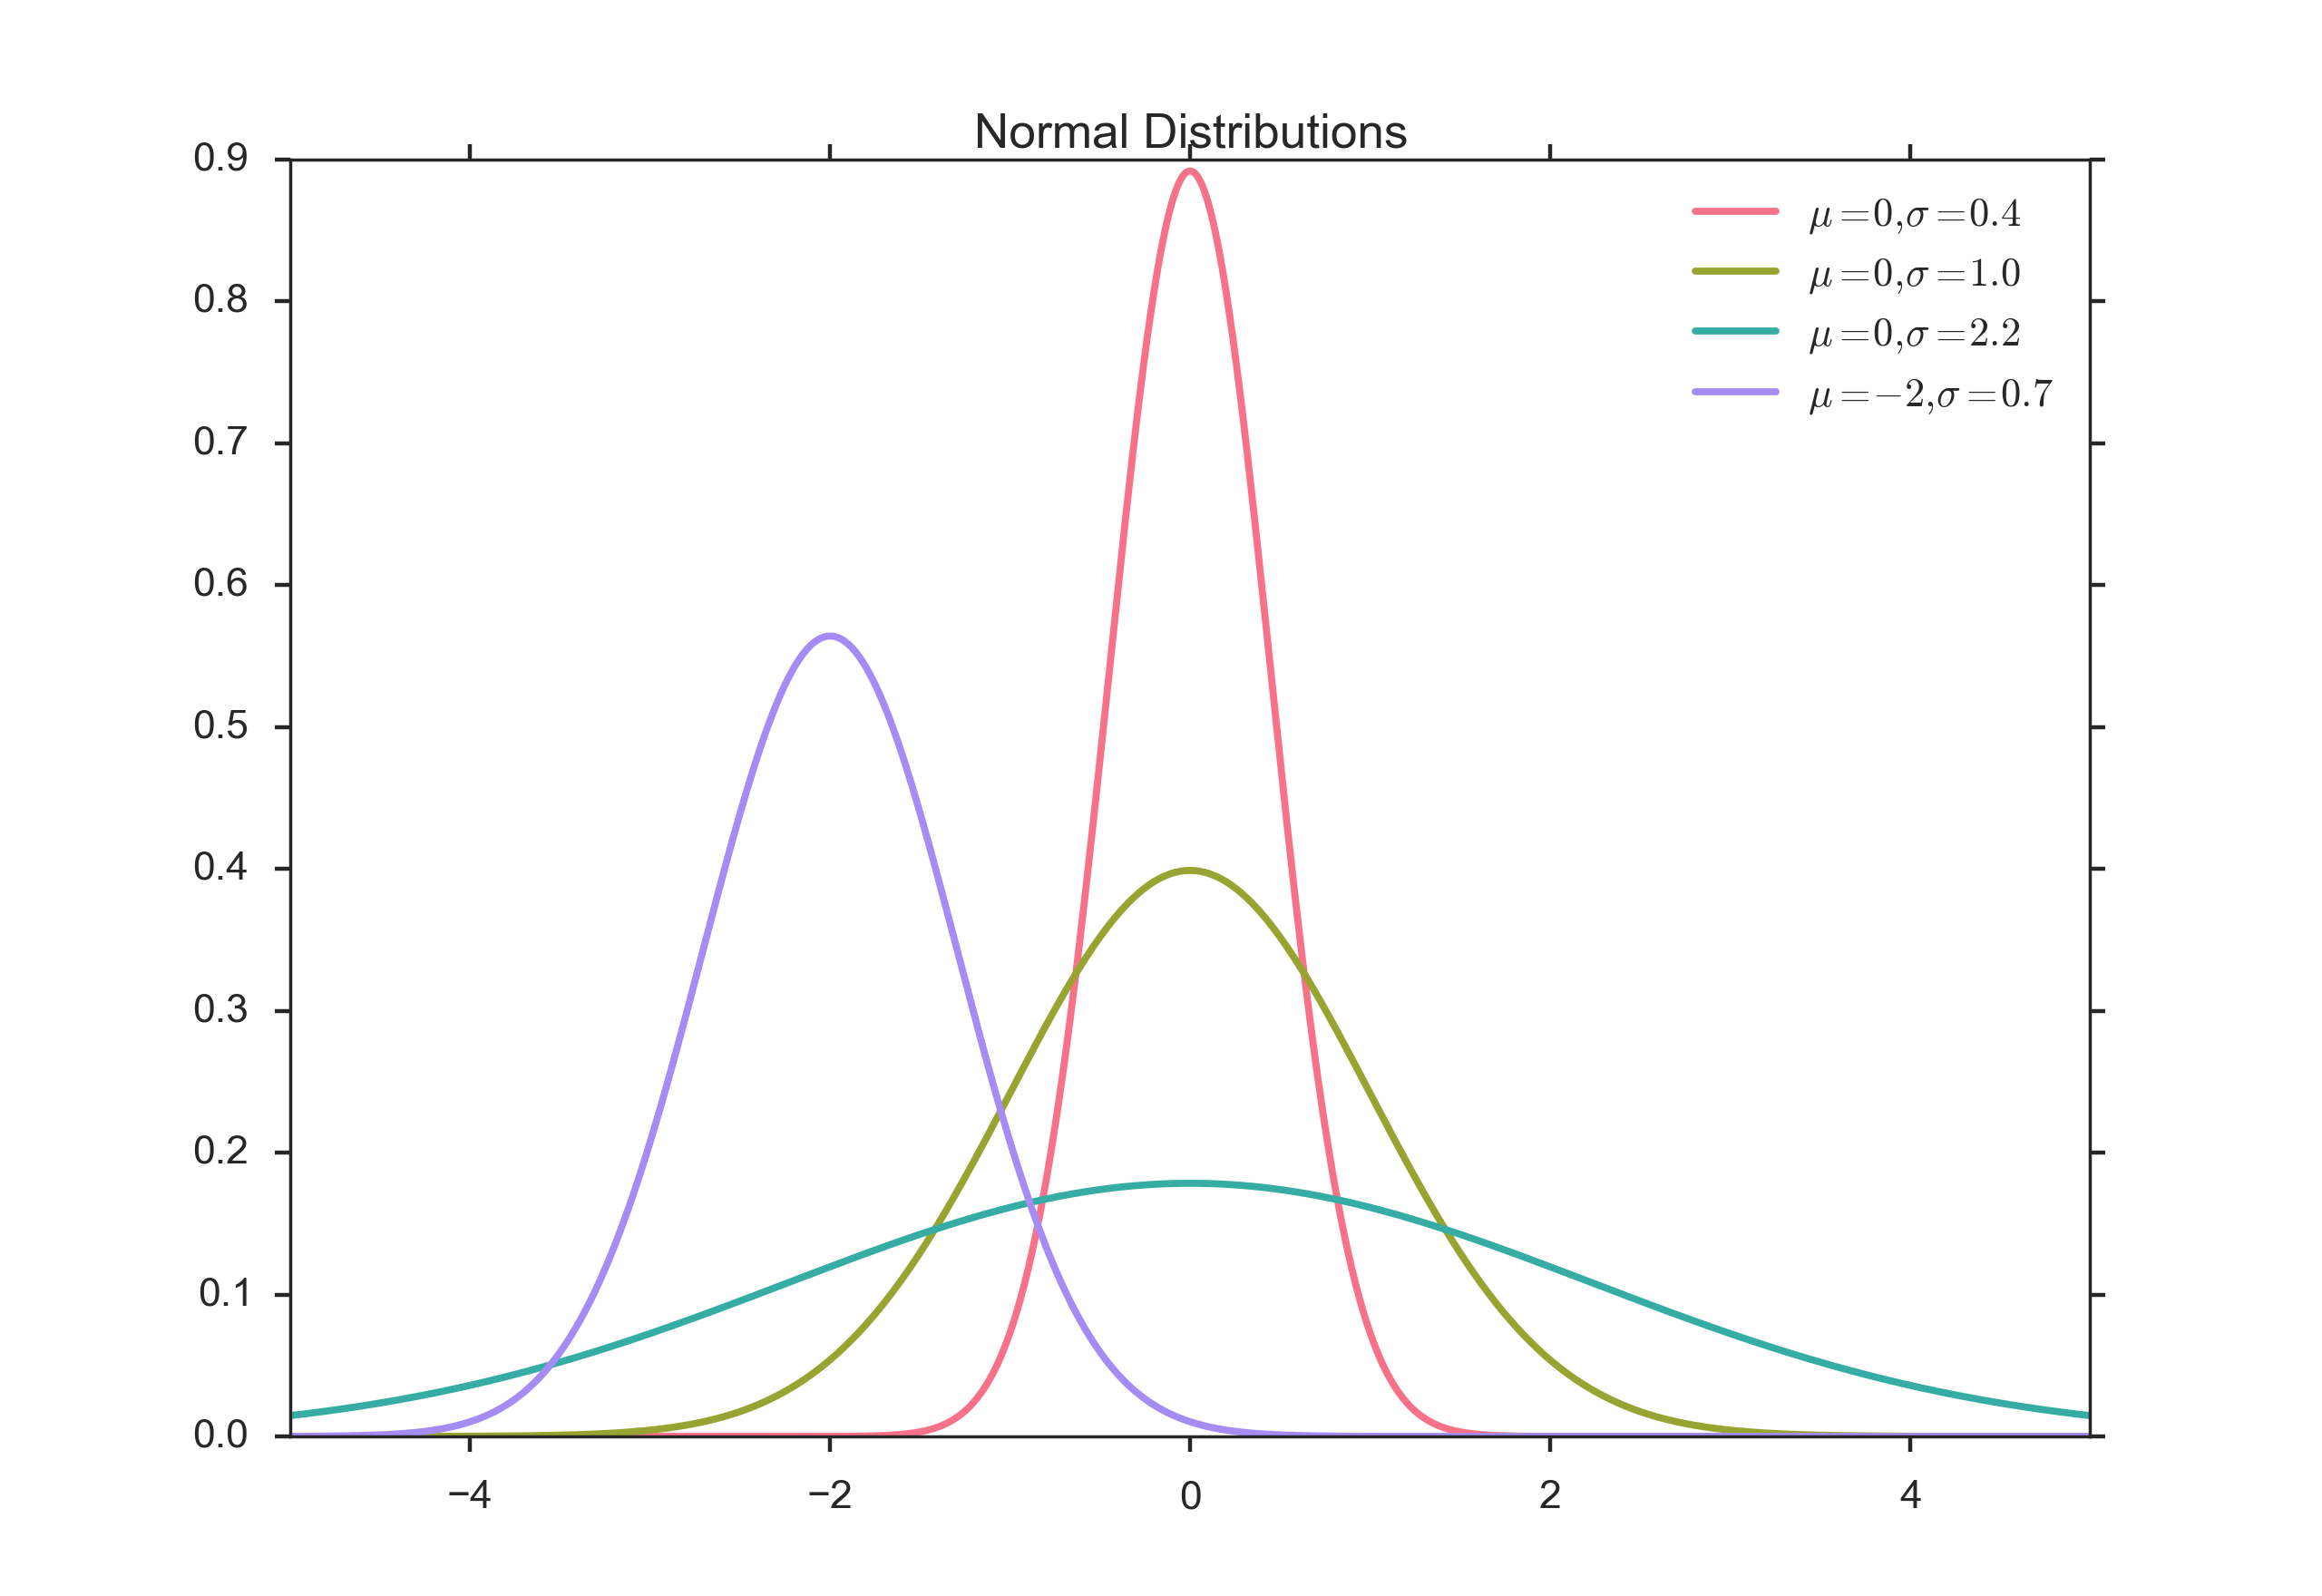
\includegraphics[width=0.75\textwidth]{../Images/Normal_Distribution_PDF.png}\\
  \caption{Normal Distribution}\label{fig:normal}
\end{figure}

For smaller sample numbers, the sample distribution can show quite a bit of variability. For example, look at 25 distributions generated by sampling 100 numbers from a normal distribution (Fig. \ref{fig:MultipleNormal})

\begin{figure}[h]
  \centering
  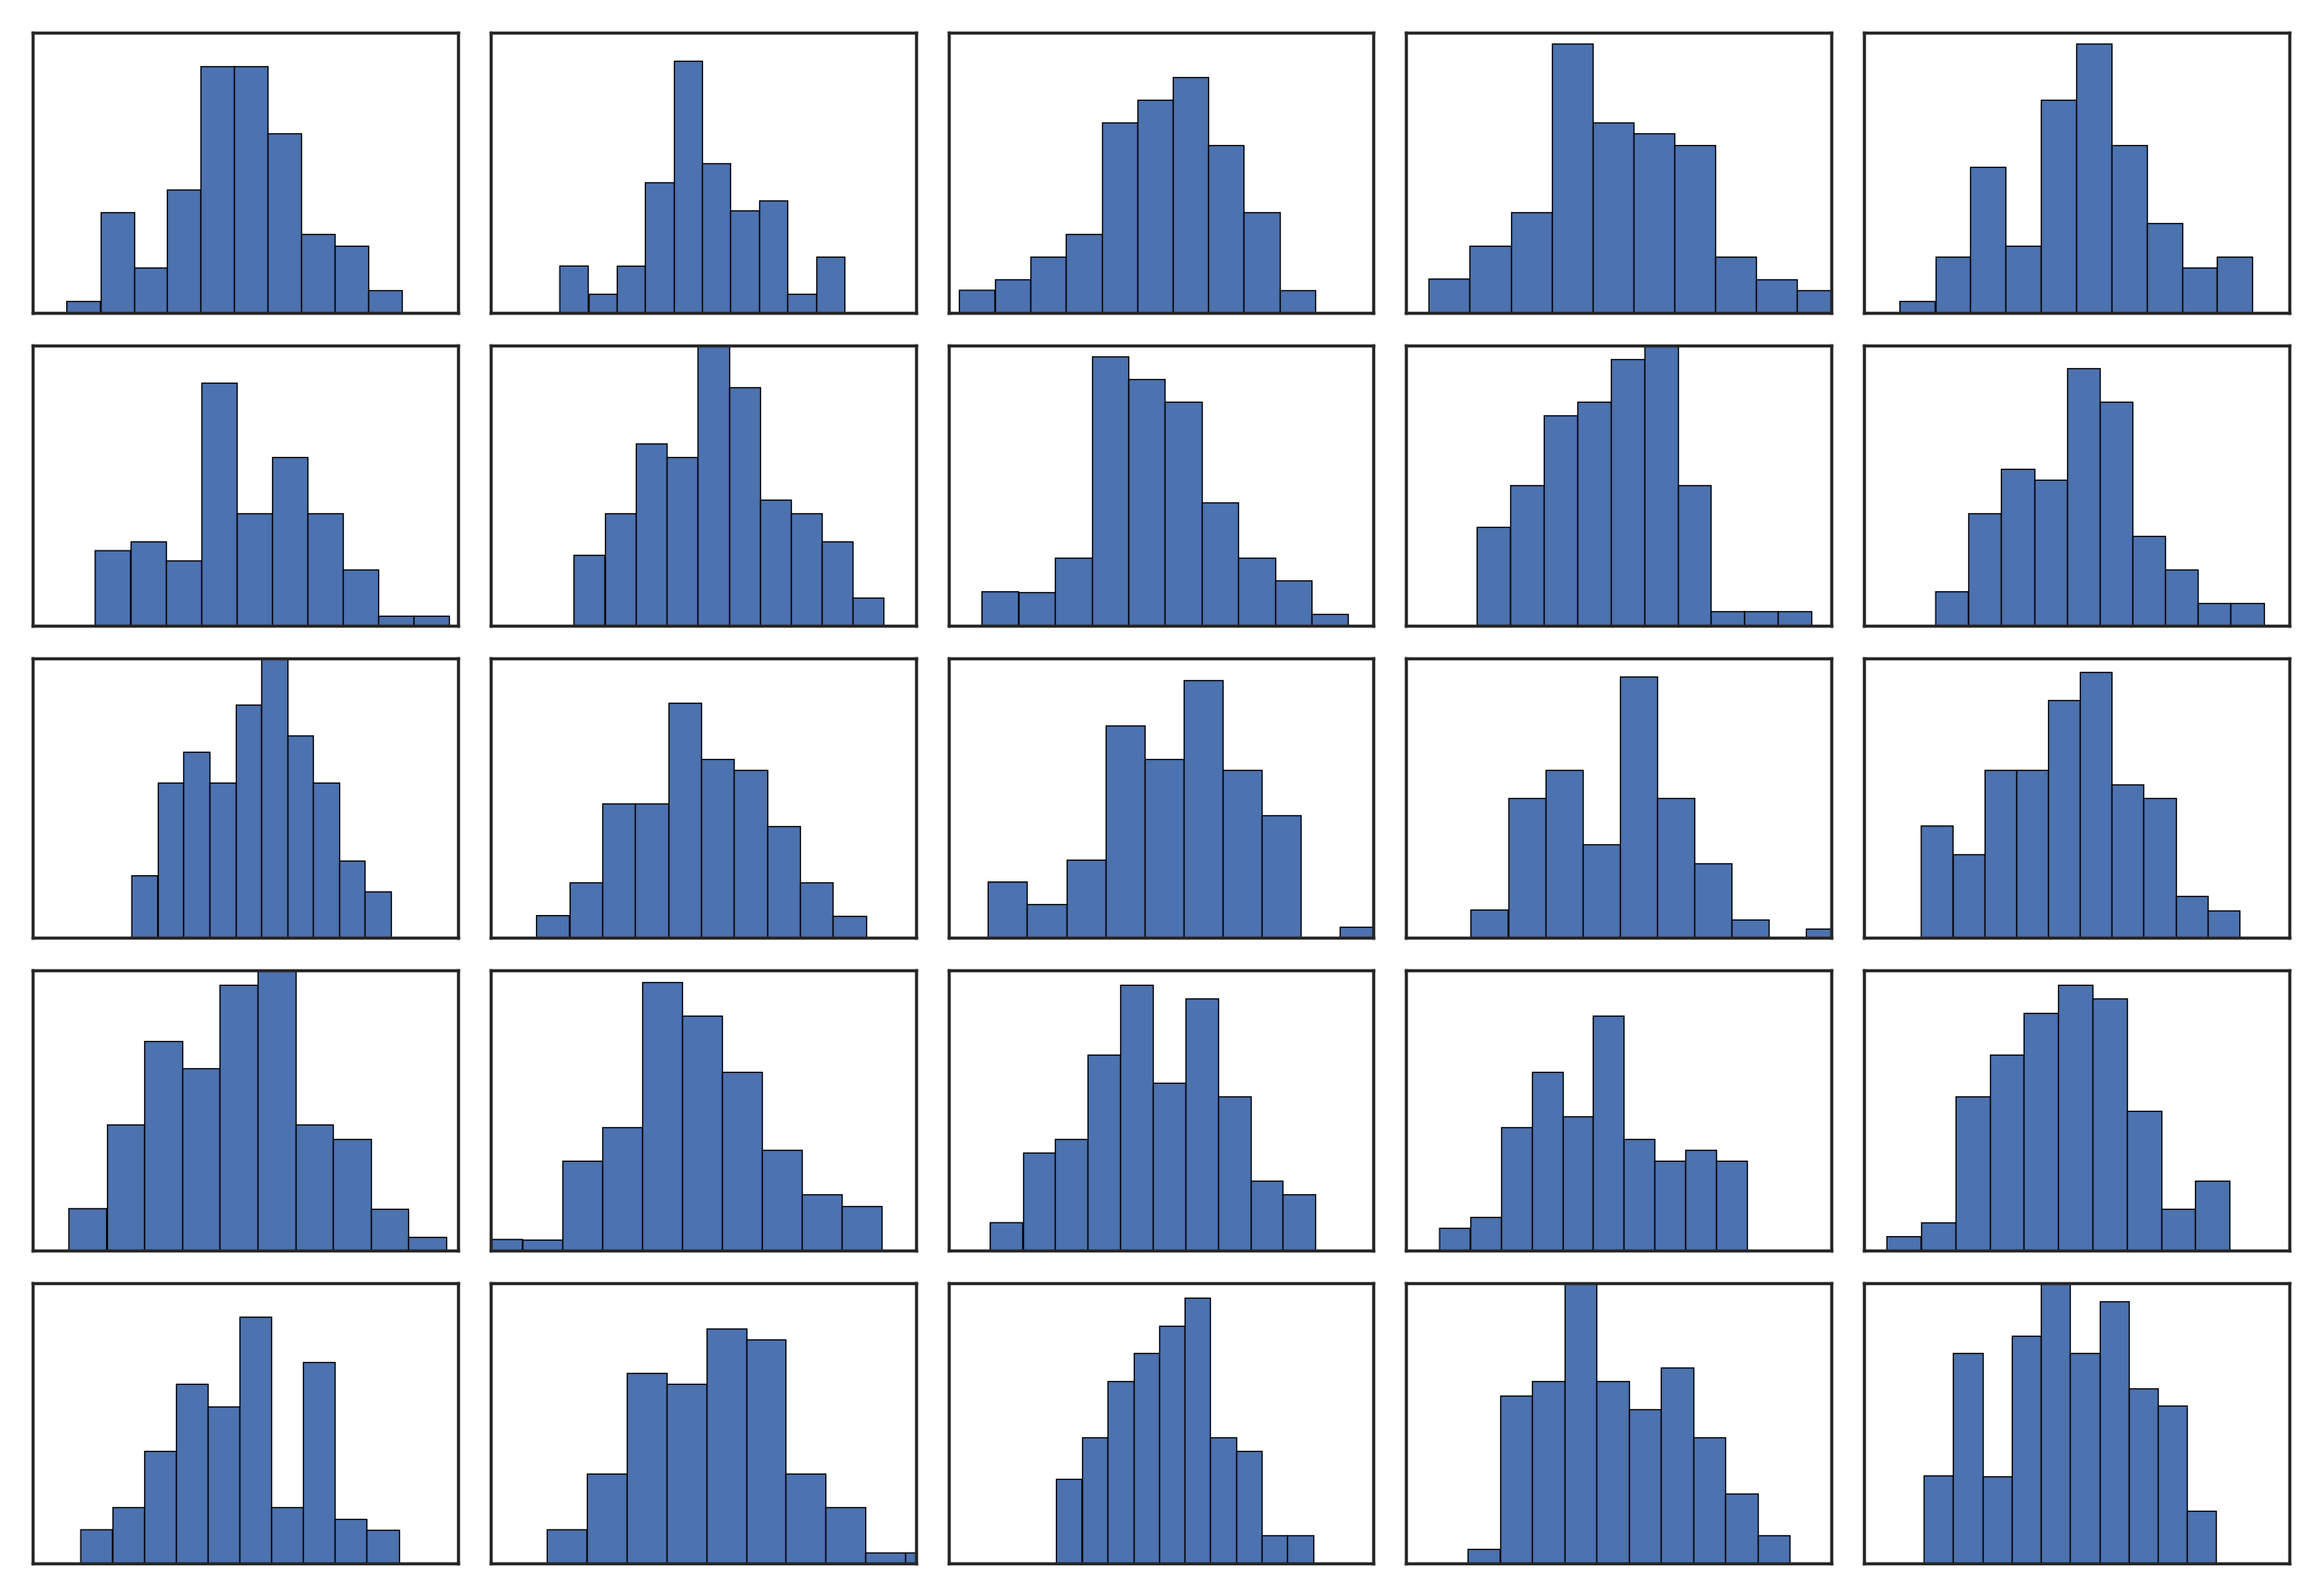
\includegraphics[width=0.75\textwidth]{../Images/Normal_MultHist.png}\\
  \caption{25 randomly generated normal distributions of 100 points.}\label{fig:MultipleNormal}
\end{figure}

Some examples of applications are:

\begin{itemize}
\item{}If the average man is 175 cm tall with a variance of 6 cm, what is the probability that a man found at random will be 183 cm tall?
\item{}If the average man is 175 cm tall with a variance of 6 cm and the average woman is 168 cm tall with a variance of 3 cm, what is the probability that the average man from a given sample will be shorter than the average woman from a given sample?
\item{}If cans are assumed to have a variance of 4 grams, what does the average weight need to be in order to ensure that the 99\% of all cans have a weight of at least 250 grams?

\end{itemize}

The normal distribution with parameters $\mu$ and $\sigma$ is denoted as {$N(\mu,\sigma)$}. If the \emph{random variate (rv)} {\itshape X} is normally distributed with expectation $\mu$ and standard deviation $\sigma$, one denotes: {$\,X \sim N(\mu,\sigma)$} or $\,X \in N(\mu,\sigma)$.

\begin{table}
  \centering
  \begin{tabular}{c c c}
    \hline
     & \multicolumn{2}{ c } {Probability of being} \\
    Range & within range & outside range \\
    \hline
    % after \\: \hline or \cline{col1-col2} \cline{col3-col4} ...
    mean $\pm$ 1SD & 0.683 & .317 \\
    mean $\pm$ 2SD & 0.954 & 0.046 \\
    mean $\pm$ 3SD & 0.9973 & 0.0027 \\
    \hline
  \end{tabular}
  \caption{Tails of a normal distribution.}
\end{table}


Figure \ref{fig:DistributionUtilities} shows a number of functions are commonly used to select appropriate points from a distribution function:

\begin{itemize}
  \item \emph{Probability density function (PDF)}: note that to obtain the probability for the variable appearing in a certain interval, you have to \emph{integrate} the PDF over that range.
  \item \emph{Cumulative distribution function (CDF)}: gives the probability of obtaining a value smaller than the given value
  \item \emph{Survival function (SF)}: 1-CDF: gives the probability of obtaining a value larger than the given value. It can also be interpreted as the proportion of data "surviving" above a certain value.
  \item \emph{Percentile point function (PPF)}: the inverse of the CDF. Answers the question "Given a certain probability, what is the corresponding value for the CDF?"
  \item \emph{Inverse survival function (ISF)}: the name says it all.
\end{itemize}

\textbf{Note:}
In Python, the most elegant way of working with distribution function is a two-step procedure:
\begin{itemize}
  \item In the first step, you create your distribution (e.g. \textsf{nd = stats.norm()}). Note that is a \emph{distribution} (in Python parlance a "frozen distribution"), not a function yet!
  \item In the second step, you decide which function you want to use from this distribution, and calculate the function value for the desired x-input (e.g. \textsf{y = nd.cdf(x)})
\end{itemize}

\PyImg "distributionNormal.py" (p \pageref{py:distributionNormal}) shows simple manipulations of normal distribution functions.
\index{python}{distributionNormal}

\begin{figure}[h]
  \centering
  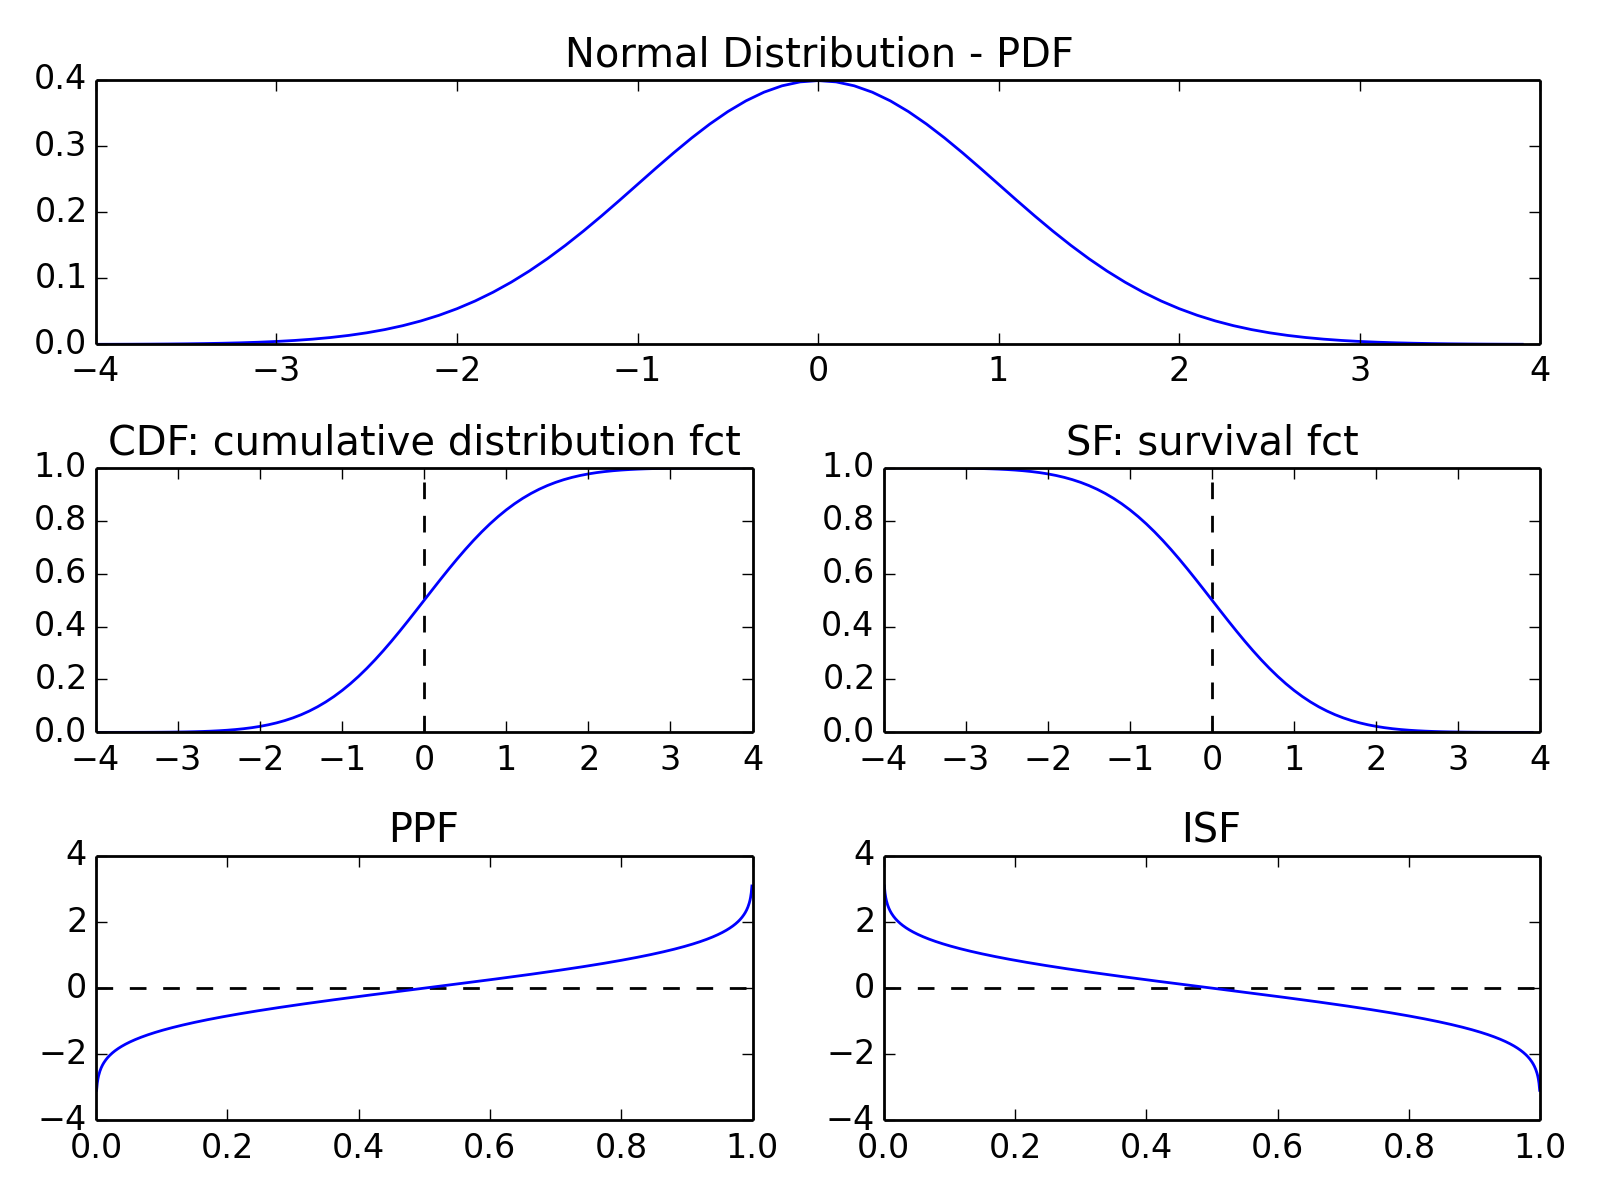
\includegraphics[width=0.75\textwidth]{../Images/DistributionFunctions.png}\\
  \caption{Utility functions for continuous distributions, here for the normal distribution.}\label{fig:DistributionUtilities}
\end{figure}

\begin{lstlisting}
  In [33]:  from scipy import stats
  In [34]:  mu = -2
  In [35]:  sigma = sqrt(0.5)
  In [36]:  myDistribution = stats.norm(mu, sigma)
  In [37]:  significanceLevel = 0.05
  In [38]:  myDistribution.ppf([significanceLevel/2, 1-significanceLevel/2])
  Out[38]:  array([-3.38590382, -0.61409618]
\end{lstlisting}
\emph{Example of how to calculate the interval of the PDF containing 95\% of the data, for the green curve in Figure \ref{fig:normal}}

\subsection{Other Continuous Distributions}\label{sec:ContinuousDistributions} \index{general}{distributions!continuous}

The distributions you will enounter most frequently are:

\begin{itemize}
  \item \textbf{Normal distribution} - the "ideal" continuous probability distribution
  \item \textbf{t-distribution} - for sample distributions (What you will probably use most often.)
  \item \textbf{$\chi$-square distribution} - for describing  variability
  \item \textbf{F-distribution} - for comparing variability
\end{itemize}

In the following, we will describe these distributions in more detail.

\subsubsection{t Distribution}\index{general}{distributions!t-distribution}
For a small number of samples (ca.$<10$) from a normal distribution, the distribution of the mean deviates slightly from the normal distribution. The reason is that the sample mean does not coincide exactly with the population mean. This modified distribution is the \emph{t-distribution}, and converges for larger values towards the normal distribution (Fig. \ref{fig:t}).

If $\bar{x}$ is the sample mean, and $s$ the sample standard deviation, then

\begin{equation}\
  t = \frac{\bar{x}-\mu}{s/ \sqrt{n}}
\end{equation}

A very frequent application of the t-distribution is in the calculation of confidence intervals (Eq. \ref{eq:ci}):

\begin{lstlisting}
  In [28]: n = 20
  In [29]: alpha = 0.05
  In [30]: stats.t(20).ppf(1-alpha/2)
  Out[30]: 2.0859634472658364

  In [31]: stats.norm.ppf(1-alpha/2)
  Out[31]: 1.959963984540054
\end{lstlisting}
\emph{Calculating the t-values for confidence intervals, for n = 20 and $\alpha=0.05$. For comparison, I also calculate the corresponding value from the normal distribution.}


\begin{figure}
  \centering
  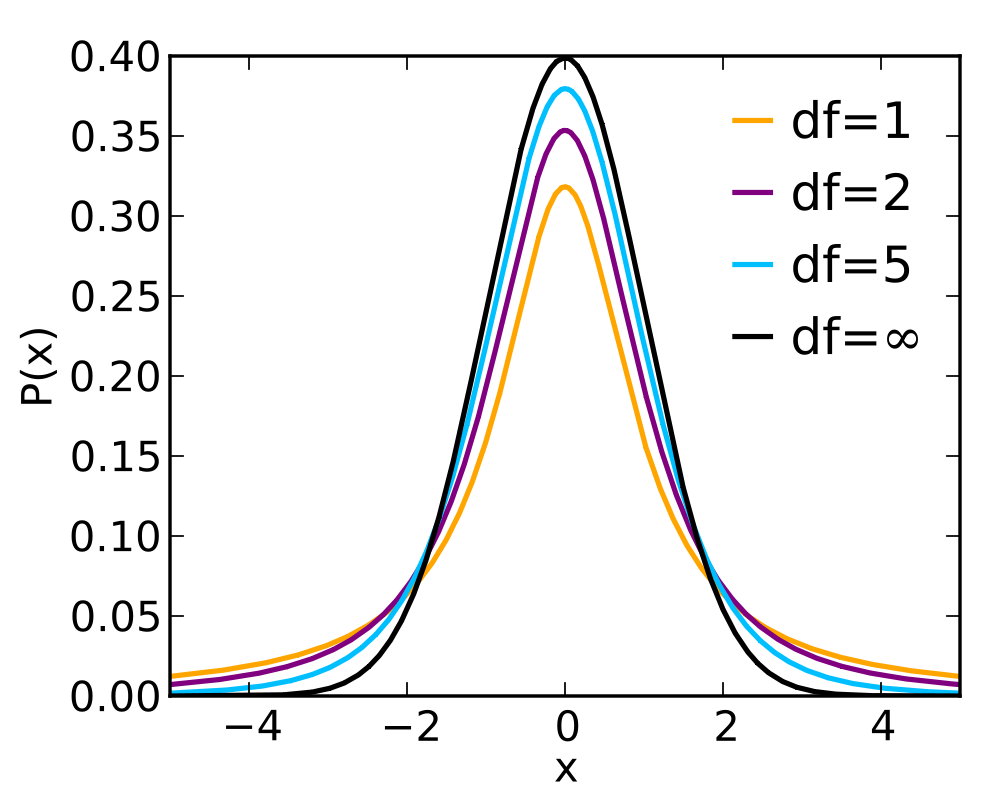
\includegraphics[width=0.5\textwidth]{../Images/Student_t_pdf.png}\\
  \caption{t Distribution}\label{fig:t}
\end{figure}


\subsubsection{Chi-square Distribution}\index{general}{distributions!chi square}

The \emph{Chi-square distribution} is related to normal distribution in a simple way: If a random variable $X$ has a normal distribution ($X \in N(0,1)$), then $X^2$ has a chi-square distribution, with one degree of freedom ($X^2 \in \chi_{1}^2$). The sum squares of $n$ independent and standard normal random variables has a chi-square distribution with $n$ degrees of freedom:

\begin{equation}
    \sum\limits_{i = 1}^n {X_i^2} \in \chi_{n}^2
\end{equation}


\begin{figure}
  \centering
  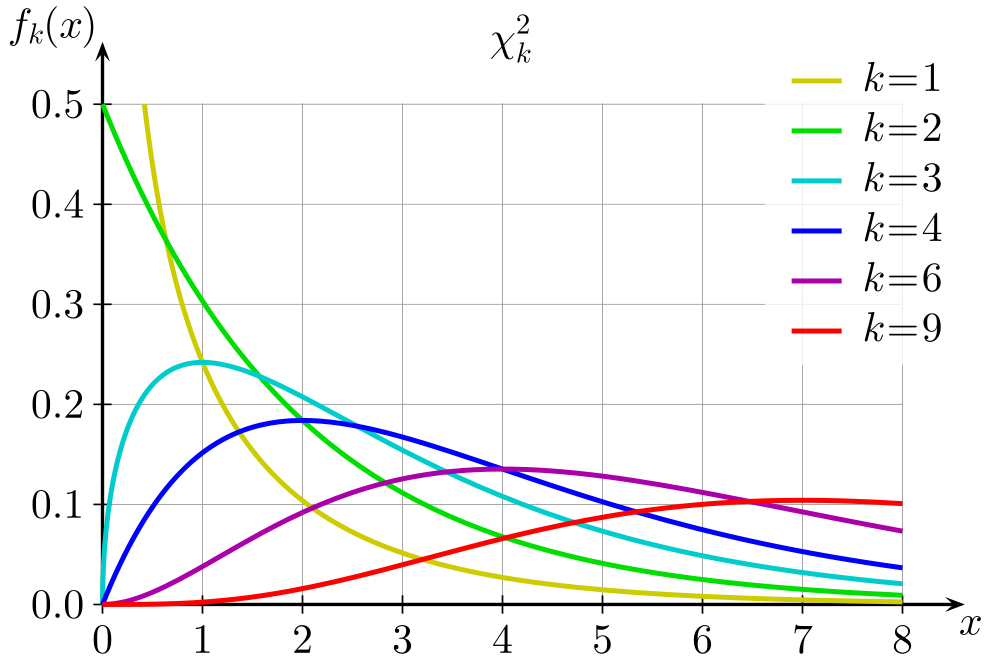
\includegraphics[width=0.5\textwidth]{../Images/ChiSquare_pdf.png}\\
  \caption{Chi-square Distribution}
\end{figure}


\subsubsection{F Distribution}\index{general}{distributions!F distribution}
Named after Sir Ronald Fisher, who developed the F distribution for use in determining critical values in ANOVAs (\emph{ANalysis Of VAriance}).  The cutoff values in an F table are found using three variables:

\begin{itemize}
  \item ANOVA numerator degrees of freedom
  \item ANOVA denominator degrees of freedom
  \item significance level
\end{itemize}

ANOVA compares the size of the variance between two different samples. This is done by dividing the larger variance over the smaller variance. The formula for the resulting \emph{F statistic} is:

\begin{equation}
    F(r_1, r_2) = \frac{\chi_{r1} ^2 /r_1}{\chi_{r2} ^2 /r_2}
\end{equation}

where $\chi_{r1}^2$ and $\chi_{r2}^2$ are the chi-square statistics of sample one and two respectively, and $r_1$ and $r_2$ are their degrees of freedom, i.e. the number of observations.

\paragraph{F-Test of Equality of Variances}
If you want to investigate whether two groups have the same variance, you have to calculate the ratio of the sample standard deviations squared:

\begin{equation}
  F = \frac{S_x^2}{S_y^2}
\end{equation}

where $S_x$ ist he sample standard deviation of the first sample, and $S_y$ the sample standard deviation for the second sample.

One example could be if you want to compare apples that look alike but are from different trees and have different sizes. There are three apples from the first tree that weigh 110, 121 and 143 grams respectively, and four from the other which weigh 88, 93, 105 and 124 grams respectively. The F statistic is $F = 1.05$, and has $n-1$ and $m-1$ degrees of freedom, where $n$ and $m$ are the number of apples in each batch. The code sample below shots what the F statistic is close to the center of the distribution, so we cannot reject the hypothesis that the two batches have the same variance.

\begin{lstlisting}
  In [1]:  apples1 = array([110, 121, 143])
  In [2]:  apples2 = array([88, 93, 105, 124])
  In [3]:  fval = std(apples1, ddof=1)/std(apples2, ddof=1)
  In [4]:  fd = stats.f(2,3)
  In [5]:  p = fd.cdf(fval)
  In [6]:  print p
  Out[6]:  0.548708891481
  In [7]:  if (p<0.025) or (p>0.975):
              print 'There is a significant difference between the two distributions.'
\end{lstlisting}

\begin{figure}
  \centering
  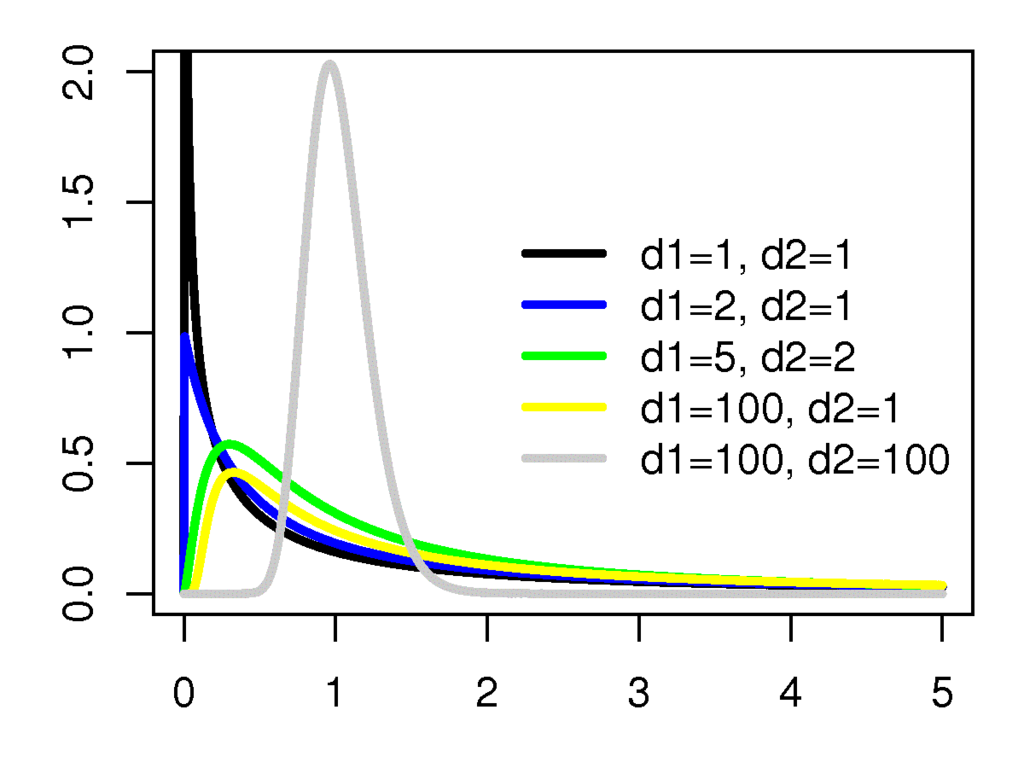
\includegraphics[width=0.5\textwidth]{../Images/F_distributionPDF.png}\\
  \caption{F Distribution}
\end{figure}


\subsubsection{Lognormal Distribution}\index{general}{distributions!lognormal}

In some circumstances a set of data with a positively skewed distribution can be transformed into a symmetric distribution by taking logarithms. Taking logs of data with a skewed distribution will often give a distribution that is near to normal (see Figure \ref{fig:lognormal}).

\begin{figure}
\centering
\begin{subfigure}{.5\textwidth}
  \centering
  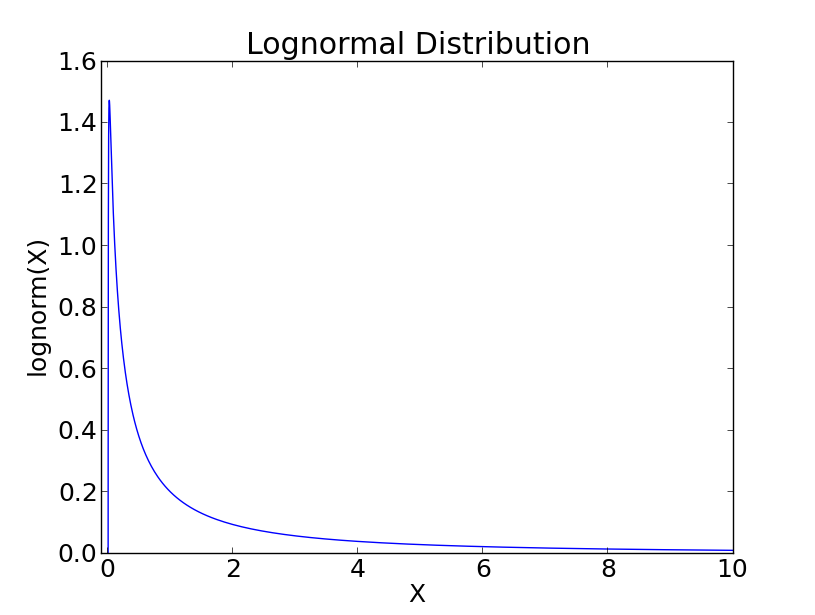
\includegraphics[width=.8\linewidth]{../Images/LogNormal_Linear.png}
  \caption{Plotted against a linear abscissa.}
  \label{fig:Lognormal_Sub1}
\end{subfigure}%
\begin{subfigure}{.5\textwidth}
  \centering
  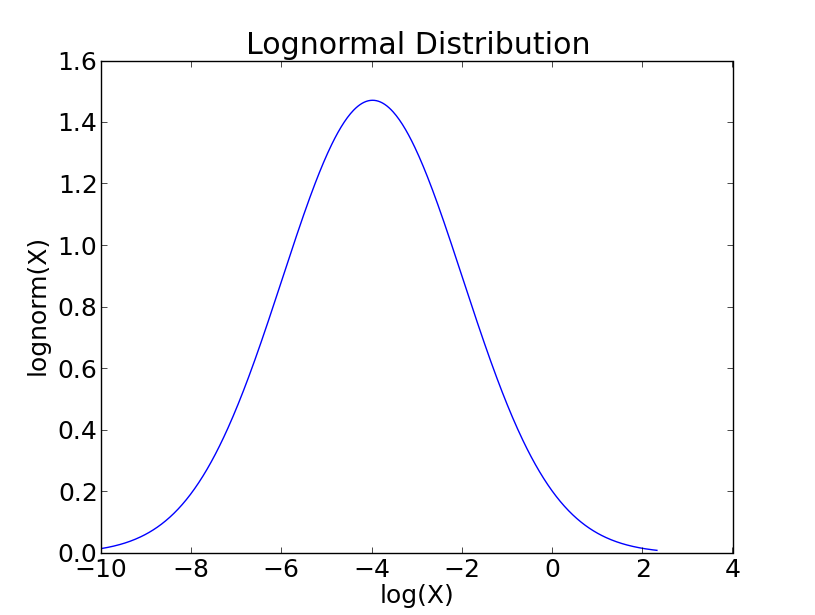
\includegraphics[width=.8\linewidth]{../Images/LogNormal_Logarithmic.png}
  \caption{Plotted against a logarithmic abscissa.}
  \label{fig:Lognormal_Sub2}
\end{subfigure}
\caption{Lognormal distribution}
\label{fig:lognormal}
\end{figure}

\subsubsection{Weibull Distribution}\index{general}{distributions!weibull}

The Weibull distribution is the most commonly used distribution for modeling reliability data or "survival" data. It has two parameters, which allow it to handle increasing, decreasing or constant failure-rates (see Figure \ref{fig:weibull}).
It is defined as

\begin{equation}\label{eq_weibull}
f_x (x) =
  \begin{cases}
    \frac{k}{\lambda}\left(\frac{x}{\lambda}\right)^{k-1}e^{-(x/\lambda)^{k}} & x\geq0 ,\\
    0 & x<0 ,
    \end{cases}
\end{equation}

where $k > 0$ is the \emph{shape parameter }and $\lambda > 0$ is the \emph{scale parameter }of the distribution. Its complementary cumulative distribution function is a stretched exponential function.

If the quantity x is a "time-to-failure", the Weibull distribution gives a distribution for which the failure rate is proportional to a power of time. The shape parameter, k, is that power plus one, and so this parameter can be interpreted directly as follows:

\begin{itemize}
  \item  A value of $k < 1$ indicates that the failure rate decreases over time. This happens if there is significant "infant mortality", or defective items failing early and the failure rate decreasing over time as the defective items are weeded out of the population.

  \item  A value of $k = 1$ indicates that the failure rate is constant over time. This might suggest random external events are causing mortality, or failure.
  \item  A value of $k > 1$ indicates that the failure rate increases with time. This happens if there is an "aging" process, or parts that are more likely to fail as time goes on.
\end{itemize}

In the field of materials science, the shape parameter k of a distribution of strengths is known as the Weibull modulus.

\begin{figure}
  \centering
  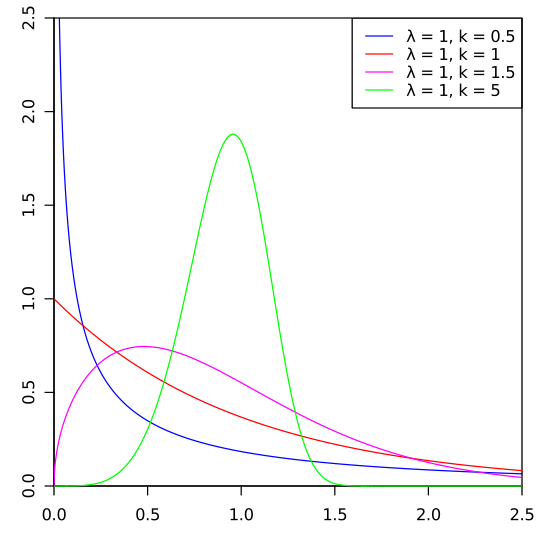
\includegraphics[width=0.5\textwidth]{../Images/Weibull_PDF.png}\\
  \caption{Weibull Distribution}\label{fig:weibull}
\end{figure}


\subsubsection{Exponential Distribution}\index{general}{distributions!exponential}

For a stochastic variable X with an \emph{exponential distribution}, the probability distribution function is:
\begin{equation}\label{eq_exponential}
f_x (x) =
  \begin{cases}
\lambda e^{- \lambda x}, & \mbox{if } x \ge 0 \\
0, & \mbox{if } x < 0
\end{cases}
\end{equation}

The exponential PDF is shown in Figure \ref{fig:exponential}
\begin{figure}
  \centering
  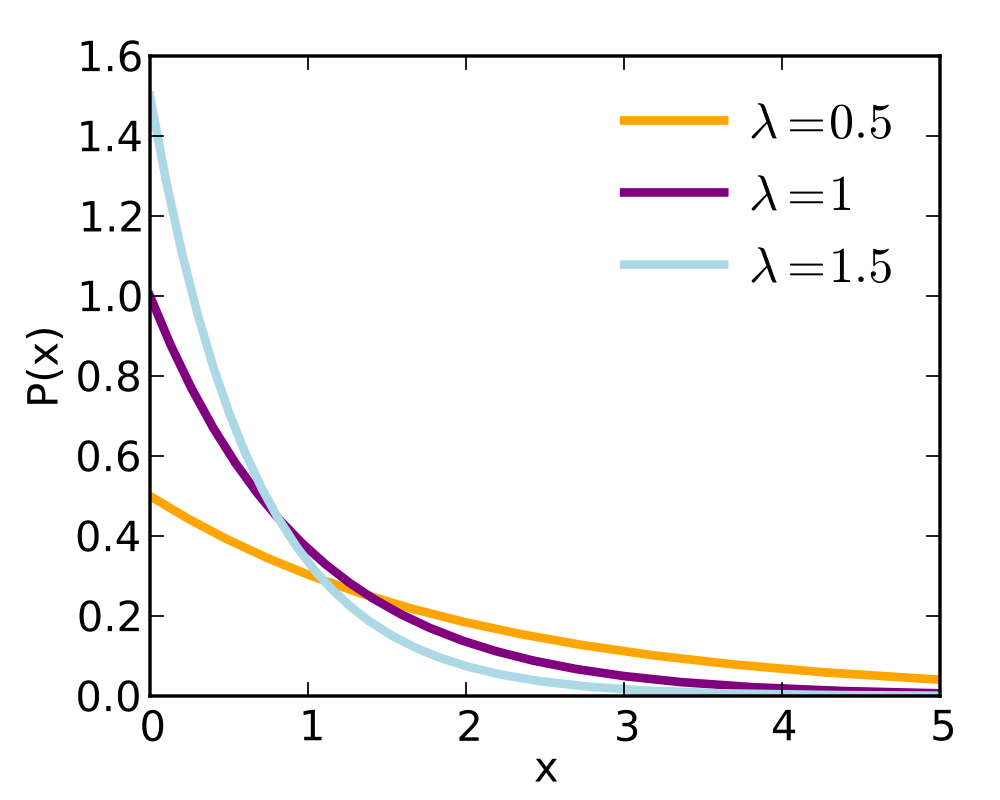
\includegraphics[width=0.5\textwidth]{../Images/Exponential_pdf.png}\\
  \caption{Exponential Distribution}\label{fig:exponential}
\end{figure}


\subsubsection{Uniform Distribution}\index{general}{distributions!uniform}

This is a simple one: an even probability for all data values (Figure \ref{fig:uniform}). Not very common for real data.

\begin{figure}
  \centering
  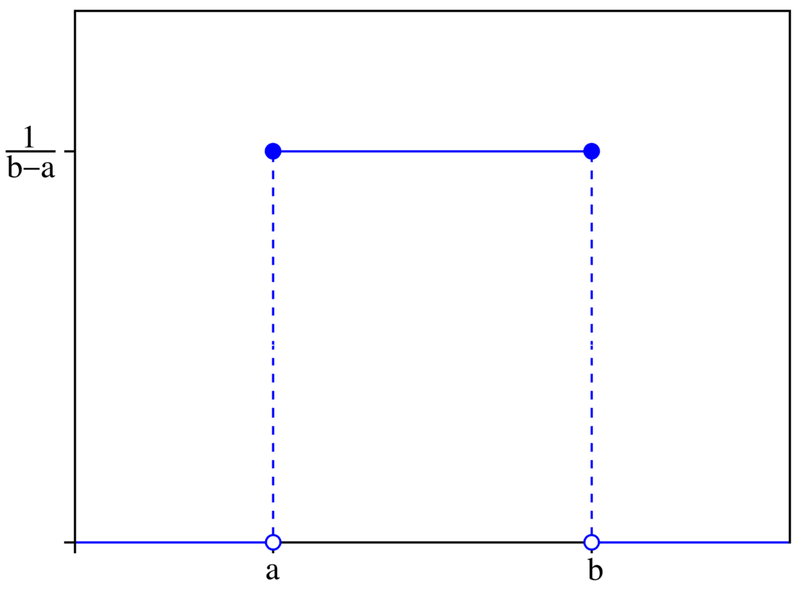
\includegraphics[width=0.5\textwidth]{../Images/Uniform_Distribution_PDF.png}\\
  \caption{Uniform Distribution} \label{fig:uniform}
\end{figure}

\subsubsection{Programs: Continuous Distribution Functions}

Working with distribution functions in Python takes a bit to get used to. But once you get the concept, it is marvellously easy. In my opinion, the most logical way is first to define the function, with all the parameters that it requires; and then, to use the methods of this function, e.g. $pdf$, or $cdf$:

\begin{lstlisting}
  In [1]: from scipy import stats
  In [2]: myDF = stats.norm(5,3)
  In [3]: x = linspace(-5, 15, 101)
  In [4]: y = myDF.pdf(x)
\end{lstlisting}

\PyImg "distributionContinuous.py" (p \pageref{py:continuous}) shows different continuous distribution functions.
\index{python}{distributionContinuous}

\subsection{Discrete Distributions}\index{general}{distributions!discrete}

While the functions describing continuous distributions are referred to as \emph{probability density functions}, discrete distributions are described by \emph{probability mass functions}.

\subsubsection{Binomial Distribution}\index{general}{distributions!binomial}
The Binomial is associated with the question "Out of a given number of trials, how many will succeed?" Some example questions that are modeled with a Binomial distribution are:
\begin{itemize}
  \item Out of ten tosses, how many times will this coin land ''heads''?
  \item From the children born in a given hospital on a given day, how many of them will be girls?
  \item How many students in a given classroom will have green eyes?
  \item How many mosquitos, out of a swarm, will die when sprayed with insecticide?
\end{itemize}

  We conduct $n$ repeated experiments where the probability of success is given by the parameter $p$ and add up the number of successes. This number of successes is represented by the random variable $X$.  The value of $X$ is then between 0 and $n$.

When a random variable X has a Binomial Distribution with parameters $p$ and $n$ we write it as $\,X \sim Bin(n,p)$ or $\,X \sim B(n,p)$ and the probability mass function is given at $X=k$ by the equation:

\begin{equation}
    P\left[X = k\right] = \begin{cases} {n \choose k} p^k \left(1-p\right)^{n-k}\ & 0 \le k \le n \\ 0 & \mbox{otherwise} \end{cases} \quad 0 \leq p \leq 1, \quad n \in \mathbb{N}
\end{equation}

where ${n \choose k}={n! \over k!(n-k)!}$

\begin{figure}
  \centering
  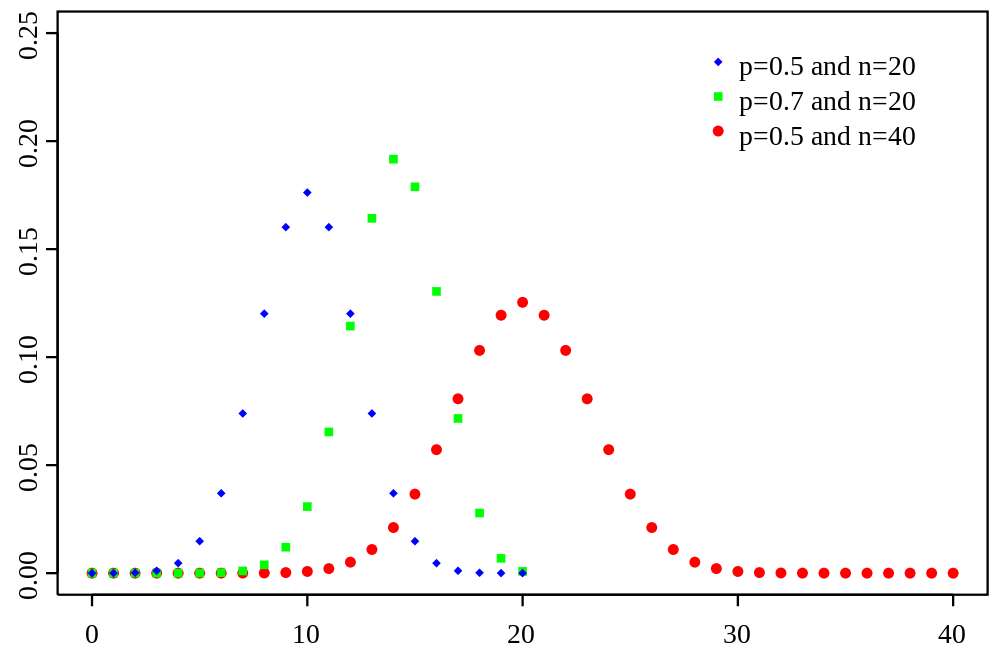
\includegraphics[width=0.75\textwidth]{../Images/Binomial_distribution_pmf.png}\\
  \caption{Binomial Distribution}
\end{figure}

The binomial distribution for $n = 1$ is sometimes referred to as \emph{Bernoulli Distribution}. \index{general}{distributions!Bernoulli}

\subsubsection{Poisson Distribution}\index{general}{distributions!poisson}

Any French speaker will notice that "Poisson" means "fish", but really there's nothing fishy about this distribution. It's actually pretty straightforward. The name comes from the mathematician Siméon-Denis Poisson (1781-1840).

The Poisson Distribution is ''very similar'' to the Binomial Distribution. We are examining the number of times an event happens. The difference is subtle. Whereas the Binomial Distribution looks at how many times we register a success over a fixed total number of trials, the Poisson Distribution measures how many times a discrete event occurs, over a period of continuous space or time. There isn't a "total" value n. As with the previous sections, let's examine a couple of experiments or questions that might have an underlying Poisson nature.

\begin{itemize}
  \item How many pennies will I encounter on my walk home?
  \item How many children will be delivered at the hospital today?
  \item How many products will I sell after airing a new television commercial?
  \item How many mosquito bites did you get today after having sprayed with insecticide?
  \item How many defects will there be per 100 metres of rope sold?
\end{itemize}

What's a little different about this distribution is that the random variable $X$ which counts the number of events can take on \emph{any non-negative integer} value. In other words, I could walk home and find no pennies on the street. I could also find one penny. It's also possible (although unlikely, short of an armored-car exploding nearby) that I would find 10 or 100 or 10,000 pennies.

Instead of having a parameter p that represents a component probability like in the Binomial distribution, this time we have the parameter "lambda" or $\lambda$ which represents the "average or expected" number of events to happen within our experiment. The probability mass function of the Poisson is given by

\begin{equation}
  P(X=k)=\frac{e^{-\lambda}\lambda^k}{k!}
\end{equation}.


\begin{figure}
  \centering
  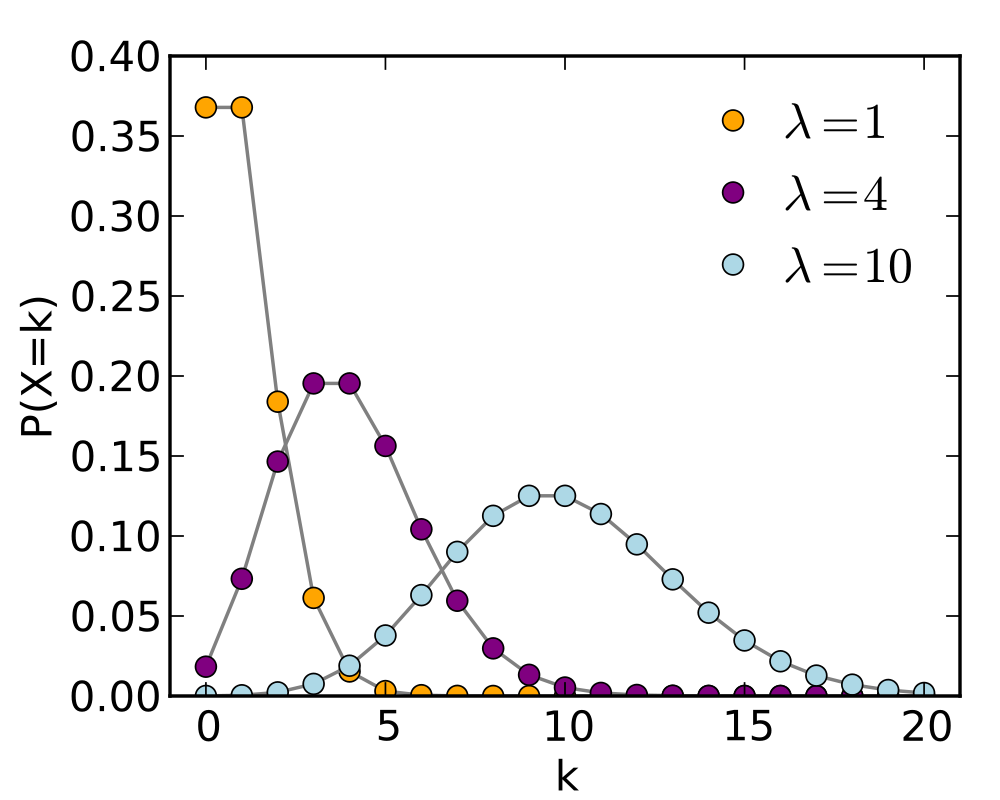
\includegraphics[width=0.5\textwidth]{../Images/Poisson_pmf.png}\\
  \caption{Poisson Distribution}
\end{figure}

\subsubsection{Programs: Discrete Distribution Functions} \index{general}{distributions!discrete}

\PyImg "distributionDiscrete.py" (p \pageref{py:discrete}) shows different continuous distribution functions.
\index{python}{distributionDiscrete}
%(Lecture 7)

\section{Data Analysis}

\subsection{Data Screening}

The first thing you have to do for your data analysis is simply \emph{look at your data}. You should check for \emph{missing data} in your data set, and \emph{outliers} which can significantly influence the result of your analysis.

\subsection{Normality Check} \index{general}{normality check}

Many statistical tests already assume that your data are normally
distributed, i.e. that they are linearly related to the standard normal
distribution. If you use any of these tests, you first have to check this assumption.

\subsubsection{QQ-Plots}\index{general}{plots!$Q-Q$ plot}

 In statistics, \emph{$Q–Q$ plots} ("Q" stands for quantile) are used for visual assessments of distributions. They are a graphical method for comparing two probability distributions by plotting their quantiles against each other. First, the set of intervals for the quantiles are chosen. A point $(x,y)$ on the plot corresponds to one of the quantiles of the second distribution (y-coordinate) plotted against the same quantile of the first distribution (x-coordinate). Thus the line is a parametric curve with the parameter which is the (number of the) interval for the quantile.

If the two distributions being compared are similar, the points in the $Q-Q$ plot will approximately lie on the line $y = x$. If the distributions are linearly related, the points in the $Q-Q$ plot will approximately lie on a line, but not necessarily on the line $y = x$ (Figure \ref{fig:qqplot}).

\begin{figure}
  \centering
  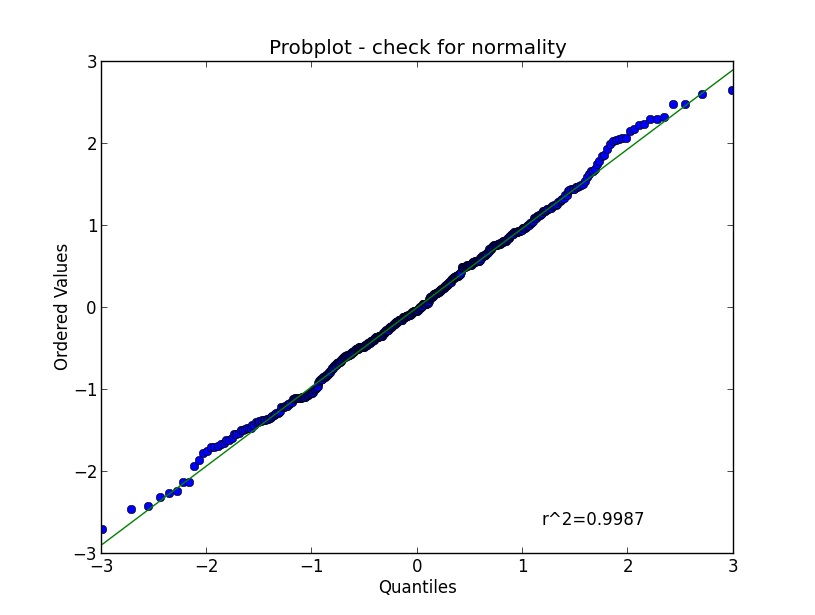
\includegraphics[width=0.75\textwidth]{../Images/ProbPlot.png}\\
  \caption{QQ-Plot, to check for normality of distribution.}\label{fig:qqplot}
\end{figure}

\subsubsection{Kolmogorov-Smirnov Test}\index{general}{test!Kolmogorov-Smirnov}

In addition, there are quantitative tests for normality. The test that I have encountered most frequently in recent literature is the \emph{Kolmogorov-Smirnov test}. The Kolmogorov-Smirnov statistic quantifies a distance between the empirical distribution function of the sample and the cumulative distribution function of the reference distribution, or between the empirical distribution functions of two samples. Note that this implies that in a test for normality, you have to i) standardize your sample distribution (i.e. subtract the mean, and divide by the standard deviation), and specify your reference distribution (i.e. if you want to check for normality, the normal distribution).

Another thest for normality is the \emph{Lilliefors test}\index{general}{test!Lilliefors}. It is a normality test based on the Kolmogorov–Smirnov test, and is used to test the null hypothesis that data come from a normally distributed population, when the null hypothesis does not specify which normal distribution; i.e., it does not specify the expected value and variance of the distribution.

Altman mainly uses the \emph{Shapiro-Wilk W test} \cite{altman99}\index{general}{test!Shapiro-Wilk}, and a number of other tests are also available.

\PyImg "checkNormality.py" (p \pageref{py:checkNormality}) shows graphical and quantitative check, if a given distribution is normal.
\index{python}{checkNormality}

\begin{figure}
  \centering
  % Requires \usepackage{graphicx}
  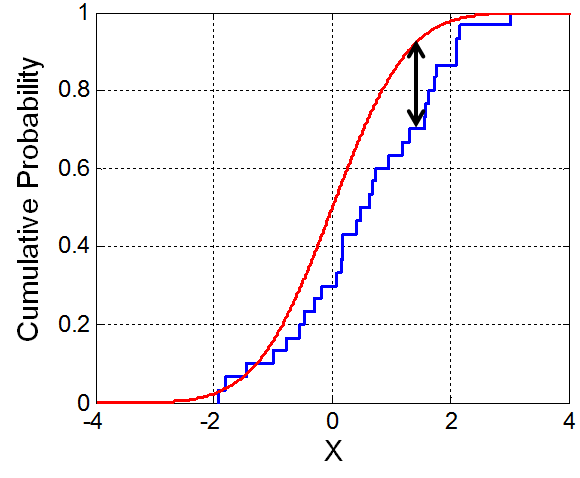
\includegraphics[width=0.5\textwidth]{../Images/KS_Example.png}\\
  \caption{Illustration of the Kolmogorov-Smirnoff statistic. Red line is CDF, blue line is an ECDF, and the black arrow is the K-S statistic (from Wikipedia).}\label{fig:ksplot}
\end{figure}


\subsection{Transformation} \index{general}{transformation}
If your data deviate significantly from a normal distribution, it is sometimes possible to make the distribution approximately normal by transforming your data. For example, data often have values that can only be positive (e.g. the size of persons), and that have  long positive tail: such data can often be made normal by applying a \emph{log transform}. This is demonstrated in Figure \ref{fig:lognormal}.

\subsection{Confidence Intervals}\index{general}{confidence interval}
Although it is common to concentrate the analysis on the p-values, it is often much more informative to report the \emph{confidence intervals} for your data. The confidence intervals are given by

\begin{equation}
  ci = mean \pm se * t_{n,\alpha}
\end{equation}\label{eq:ci}

where $se$ is the standard error, and $t_{n,\alpha}$ the $t$ statistic for $n$ degrees of freedom. For the 95\% two-sided confidence intervals, for example, you have to set $\alpha=0.025$ and $\alpha=0.975$ .

\section{Exercises}

\subsection{Python}
\begin{enumerate}
  \item Create an numpy-array, containing the data 1,2,3,...,10. Calculate mean and sample(!)-standard deviation.
    (Correct answer: 3.03)
\end{enumerate}

\subsection{Distributions}


\begin{enumerate}
  \item  Generate and plot the Probability Density Function (PDF) of a normal distribution, with a mean of 5 and a standard deviation of 3.
  \item  Generate 1000 random data from this distribution.
  \item  Calculate the standard error of the mean of these data.
    (Correct answer: ca. 0.096)

  \item  Plot the histogram of these data.
  \item  From the PDF, calculate the interval containing 95\% of these data.
    (Correct answer: [ -0.88, 10.88])
\end{enumerate}

\subsection{Analysis}
\begin{enumerate}
  \item
  \begin{enumerate}
    \item Read in the data from 'Data\textbackslash amstat\textbackslash calcium.dat.txt'.
    \item Check for erroneous entries.
    \item Check the Alkaline Phosphatase levels for normality. Use a log-transform on the data, and re-check.
  \end{enumerate}

\end{enumerate}

\subsection{Continuous Distributions }
\begin{enumerate}
    \item \textbf{T-Distribution:} Measuring the weight of your collegues, you have obtained the following weights: 52, 70, 65, 85, 62, 83, 59 kg.
    Calculate the corresponding mean, and the 99\% confidence interval for the mean. Note: with n values you have n-1 DOF for the t-distribution.
    (Correct answer: 68.0 +/- 17.2 kg)

    \item \textbf{Chi-square Distribution:} Create 3 normally distributed datasets (mean = 1, SD = 1), with 1000 samples each. Then square them, sum them (so that you have 1000 data-points), and create a histogram with 100 bins. This should be similar to the curve for the Chi-square distribution, with 3 DOF (i.e. it should come down at the left, see figure below).
    \begin{figure}
      \centering
      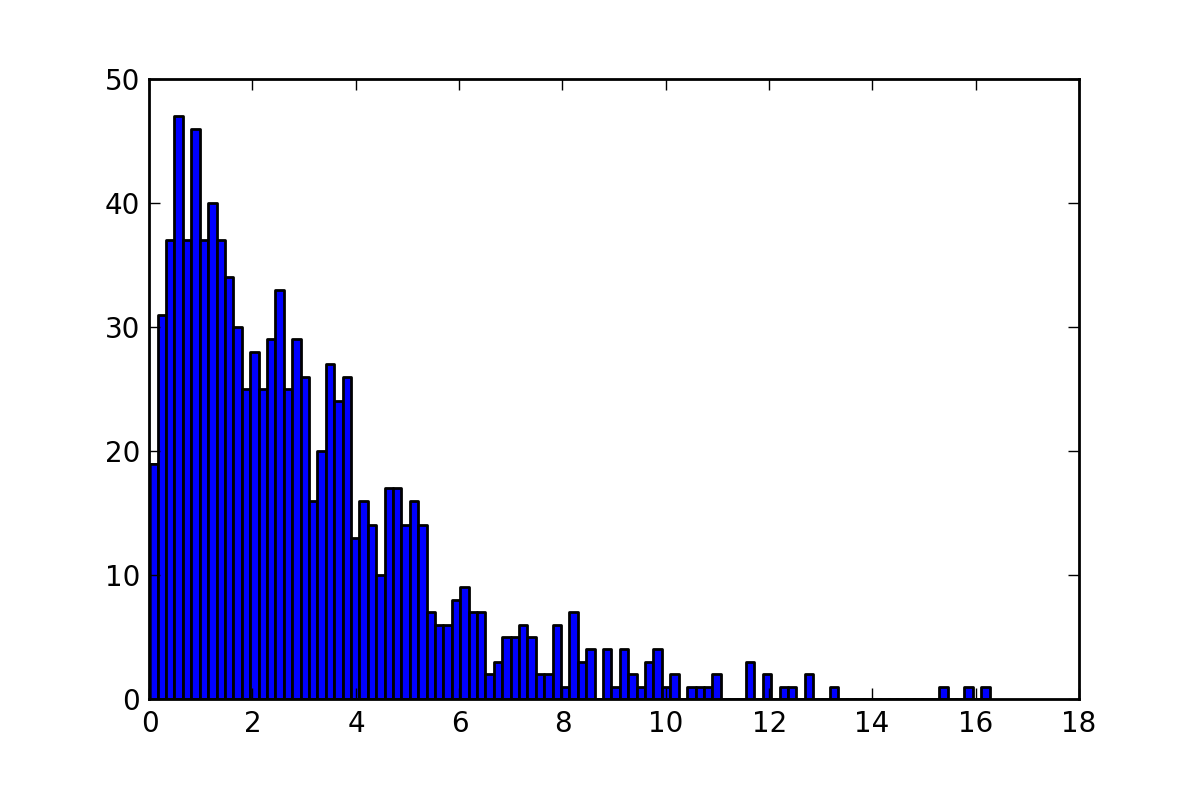
\includegraphics[width=0.5\textwidth]{../Images/chi2_3dof.png}\\
      \caption{chi2 distribution with 3 degrees of freedom.}\label{fig:chi23dof}
    \end{figure}

    \item \textbf{F Distribution:} You have two apple trees. There are three apples from the first tree that weigh 110, 121 and 143 grams respectively, and four from the other which weigh 88, 93, 105 and 124 grams respectively. Are the variances from the two trees different?
    Note: calculate the corresponding F-value, and check if the CDF for the corresponding F-distribution is $<0.025$.
    (Correct answer: no)
\end{enumerate}
\subsection{Discrete Distributions }

\begin{enumerate}
    \item \textbf{Binomial Distribution} "According to research, pure blue eyes in Europe approach greatest frequency in Finland, Sweden and Norway(at 72\%), followed by Estonia, Denmark(69\%); Latvia, Ireland(66\%); Scotland(63\%); Lithuania(61\%); The Netherlands(58\%); Belarus, England(55\%); Germany(53\%); Poland, Wales(50\%); Russia, The Czech Republic(48\%); Slovakia(46\%); Belgium(43\%); Austria, Switzerland, Ukraine(37\%); France, Slovenia(34\%); Hungary(28\%); Croatia(26\%); Bosnia and Herzegovina(24\%); Romania(20\%); Italy(18\%); Serbia, Bulgaria(17\%); Spain(15\%); Georgia, Portugal(13\%); Albania(11\%); Turkey and Greece(10\%). Further analysis shows that the average occurrence of blue eyes in Europe is 34\%, with 50\% in Northern Europe and 18\% in Southern Europe."

    If we have 15 Austrian students in the class-room, what ist the chance of finding 3, 6, or 10 students with blue eyes?
    (Correct answer: 9\%, 20.1\%, and 6.4\%)

    \item \textbf{Poisson Distribution} On the streets of Austria there were 62 fatal accidents in 2012. Assuming that those are evenly distributed, we have on average
    62 /(365/7)=1.19 fatal accidents per week. How big is the chance that in a given week there are no, 2, or 5 accidents?
    (Correct answer: 30.5\%, 21.5\%, 0.6\% )
\end{enumerate}
